\chapter{Introduction to collider experiments}  %Title of the First Chapter

\ifpdf
    \graphicspath{{Chapter1/Figs/Raster/}{Chapter1/Figs/PDF/}{Chapter1/Figs/}}
\else
    \graphicspath{{Chapter1/Figs/Vector/}{Chapter1/Figs/}}
\fi


%\section{Introduction to collider experiments}
%\label{sec:introduction}

Collider experiments are a type of particle physics experiment that involve colliding particles, typically protons or electrons, at very high energies. These collisions can lead to the creation of new particles or the detection of new phenomena, providing insight into the fundamental nature of matter. Colliders are designed to accelerate particles to nearly the speed of light and guide them along a circular or linear path using magnetic fields. By colliding particles head-on or at oblique angles, physicists can study the resulting particle showers and detect the products of the collision using complex detectors. Collider experiments have played a crucial role in advancing our understanding of particle physics and continue to be a vital tool for scientific exploration.

\section{Luminosity and its importance in particle physics}

Luminosity is a measure of the number of particle collisions that occur per unit time and per unit area. In particle physics, luminosity is a crucial parameter that determines the rate at which particles are produced in a collider experiment.

The luminosity of a collider is given by the following equation:

\begin{equation}
L = \frac{N_1 N_2 f}{A} 
\end{equation}

where $N_1$ and $N_2$ are the number of particles in each beam, f is the frequency of bunch crossings, and A is a parameter that takes into account the overlap between the two beams.

The importance of luminosity in particle physics lies in its direct relationship with the production rate of particles of interest. The production rate of a given particle is proportional to the product of the luminosity and the cross-section of the process. Thus, luminosity directly affects the ability to detect rare events and make precise measurements. The more collisions that occur, the higher the probability of rare events happening, such as the creation of new particles or the detection of new phenomena. Additionally, precise measurements require a large number of collisions to be able to statistically determine the properties of the particles being studied.

The production rate of a given particle can be expressed as:

\begin{equation}
R = L  \sigma,
\end{equation}

where R is the production rate, L is the luminosity, and $\sigma$ is the cross-section of the process that produces the particle. The cross-section is a measure of the probability that a given process will occur, and it is typically a very small number, on the order of picobarns ($10^{-36} m^2$).
In order to achieve high luminosity, particle accelerators use various techniques to increase the number of particles in the beams and focus them to a small cross-sectional area. This is done by using superconducting magnets to guide the particles along a circular path and keep them confined to a small area. Another technique is to use radio frequency cavities to accelerate the particles to higher energies increasing the frequency of bunch crossings. Increasing the number of particles in each bunch is another way to increase luminosity. In high-energy particle accelerators, such as the Large Hadron Collider (LHC) at CERN, the luminosity is typically measured in units of inverse femtobarns ($fb^{-1}$), which is a measure of the total number of collisions per unit area during the course of an experiment. For example, the LHC has a design luminosity of $10^{34} cm^{-2}s^{-1}$, which means that there are $10^{34}$ proton-proton collisions per second per square centimeter of the detector. The importance of luminosity can be seen in the many discoveries that have been made in particle physics due to high-luminosity experiments. For example, the discovery of the Higgs boson at the LHC was made possible by the high luminosity of the collider, which allowed physicists to observe the rare Higgs boson signal over the background noise of other particles. In addition to discoveries, high luminosity experiments are also important for precision measurements. For example, the measurement of the properties of the top quark, the heaviest known elementary particle, requires a large number of collisions to be able to distinguish the signal from the background noise.


\section{Motivation for precision luminosity measurement}

%One important measurement in particle physics is the measurement of the luminosity of the colliding beams. The luminosity is a measure of the number of collisions that are occurring per unit time in unit area. This measurement is important because it provides information about the rate at which rare processes occur, and it is necessary for precise measurements of cross sections and other properties of particles like couplings to fermions and bosons. The luminosity measurement with the pixel detector at the CMS experiment is a crucial measurement for the understanding of the LHC physics. The main motivation for this study is to improve the accuracy of the luminosity measurement, which is essential for many physics analyses, including searches for new particles and measurements of the properties of known particles. Luminosity uncertainty is one of the dominant uncertainty in Higgs Boson cross section and coupling measurement with other gauge bosons and fermions as shown in Fig.~\ref{fig:lum_unc}. Uncertainty in cross section and coupling measurement can not be better than uncertainty in luminosity measurement. 

In particle physics, the luminosity of colliding beams is a crucial measurement as it provides information about the rate at which rare processes occur and enables precise measurements of particle properties such as cross sections and couplings to fermions, bosons. Cross sections are fundamental quantities in particle physics, used to predict the number of events a certain process will produce. Luminosity depends on several variables, including the number of protons in each beam, the size and shape of the beams, and their relative positioning. A slight change in any of these variables can significantly alter the luminosity, which in turn affects the interpretation of collision data. Therefore, it is crucial to measure the luminosity with high precision.
%The measurement of luminosity with the pixel detector at the CMS experiment is particularly important  as it is a highly precise detector that is capable of measuring luminosity with great accuracy. It provides information about the number of charged particles passing through the detector, which is directly proportional to the number of collisions. This information is then used to calculate the luminosity. 
Improving the uncertainty in luminosity measurements is essential for many physics analyses, including searches for new particles and measurements of the properties of known particles. It is a dominant factor in the measurement of Higgs Boson cross sections and couplings to other gauge bosons and fermions, as shown in Fig~\ref{fig:lum_unc}. As such, the uncertainty in cross-section and coupling measurements cannot be better than the uncertainty in luminosity measurement. Therefore, ongoing efforts are focused on improving the accuracy of luminosity measurements, with the pixel detector at CMS being a key component of this effort. By reducing the luminosity uncertainty, physicists can make more precise measurements of particle properties and potentially discover new physics beyond the Standard Model.


%In particle physics, the luminosity of colliding beams plays a crucial role as it provides crucial data about the frequency at which rare processes take place. This enables the precise measurement of particle properties such as cross sections and couplings to fermions and bosons. Measuring luminosity with high accuracy is paramount, as it gives information about the number of charged particles that are involved in collisions. This data is then employed to determine the luminosity. Enhancing the precision of luminosity measurements is vital for numerous physics analyses, including the search for new particles and determining the properties of known particles. Luminosity uncertainty is a significant factor in the measurement of Higgs Boson cross sections and its couplings to other gauge bosons and fermions, as depicted in Fig~\ref{fig:lum_unc}. Consequently, the uncertainty in cross-section and coupling measurements cannot surpass the uncertainty in luminosity measurement. For this reason, continuous efforts are being made to increase the accuracy of luminosity measurements. By decreasing the luminosity uncertainty, physicists can achieve more accurate measurements of particle properties and potentially uncover new physics that lies beyond the confines of the Standard Model.




\begin{figure}[!htp]
\centering
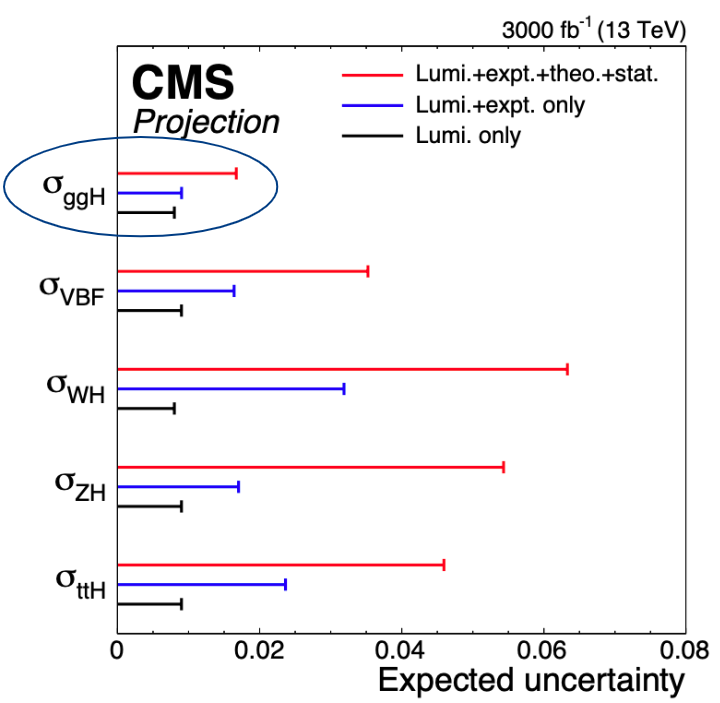
\includegraphics[width=0.42\textwidth]{ashish_thesis/lumi_precision.png}
\caption{%
   Higgs boson production processes cross section projected uncertainty. In the most precisely measured Higgs boson production process, gluon fusion (ggH), luminosity uncertainty will dominate the experimental systematic uncertainty at the High Luminosity (HL)-LHC.
}
\label{fig:lum_unc}
\end{figure}


\section{Large Hadron Collider (LHC) and the CMS Experiment}

The CERN accelerator complex consists of a series of accelerators that work together to produce beams of particles at ever-increasing energies. These beams are then fed into the LHC for further acceleration and collision. The first step in the accelerator complex is the Linac 2, a linear accelerator that produces beams of protons with an energy of 50 MeV (mega-electronvolts). The protons are then sent to the Proton Synchrotron Booster (PSB), which accelerates them to an energy of 1.4 GeV (giga-electronvolts). From there, the proton beams are sent to the Proton Synchrotron (PS), which further accelerates them to an energy of 25 GeV. The next step in the complex is the Super Proton Synchrotron (SPS), which accelerates the protons to an energy of 450 GeV. The SPS also produces beams of heavy ions, such as lead nuclei, which are used for experiments in nuclear physics and other fields. Finally, the proton beams are sent to the LHC, where they are accelerated to their maximum energy of 6.5 TeV per proton. LHC consists of a 27-kilometer ring of superconducting magnets, which guide two counter-rotating beams of protons to collide at four different locations around the ring, where four major experiments, ATLAS, the CMS (Compact Muon Solenoid) experiment, ALICE and LHCb are located as shown in Fig.~\ref{fig:lhc}. The protons are organized into "bunches," with each bunch containing around 100 billion protons. The bunches are spaced apart by 25 nanoseconds, and the LHC can contain up to 2,808 bunches per beam. The bunches in the LHC are designed to have a "bunch current" of 0.55 amperes. It uses radiofrequency (RF) cavities to accelerate the proton beams. The RF frequency used is 400 MHz, which corresponds to a wavelength of 75 centimeters. The LHC uses quadrupole magnets to focus the proton beams and keep them tightly collimated. The LHC uses a total of 1,232 superconducting dipole magnets to bend the proton beams around the circular accelerator ring. The dipole magnets are cooled to a temperature of 1.9 Kelvin (-271.3°C) using liquid helium, and are capable of producing a magnetic field of up to 8.3 tesla. The LHC's detectors record data from proton-proton collisions at a rate of around 40 million collisions per second, but only a tiny fraction of these are actually recorded for analysis. The LHC operates at a vacuum pressure of around $10^{-13}$ atmospheres, which is lower than the pressure on the surface of the moon.

\begin{figure}[!htp]
\centering
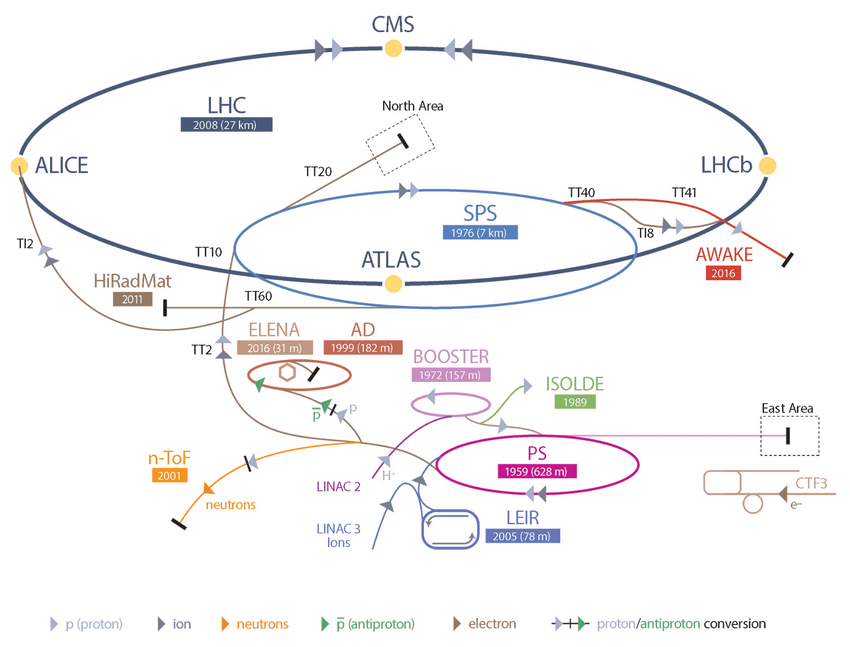
\includegraphics[width=0.6\textwidth]{ashish_thesis/lhc_schematic.png}
\caption{%
    CERN accelerator complex consists of Linac 2, Proton Synchrotron Booster (PSB), Proton Synchrotron (PS), Super Proton Synchrotron (SPS) and Large Hadron Collider (LHC). LHC ring showing four interaction points where the ALICE, ATLAS, LHCb and CMS detectors are stationed.
}
\label{fig:lhc}
\end{figure}

The CMS experiment is a multi-purpose particle detector that is designed to detect and study the particles produced in the collisions at the LHC. The CMS detector is a complex instrument that consists of several layers of sub-detectors, each designed to detect different types of particles and measure different properties of the particles.

\begin{itemize}

%\item The tracker is a key component of the Compact Muon Solenoid (CMS) detector, located at the Large Hadron Collider (LHC) at CERN. The tracker is responsible for measuring the trajectories of charged particles produced in collisions at the LHC, providing crucial information about the particles' momentum and charge. The CMS tracker consists of two main sub-detectors, the silicon pixel detector and the silicon strip tracker. The silicon pixel detector is the innermost layer of the tracker and is designed to provide precise measurements of the particles' positions. It is composed of millions of tiny silicon pixels, each capable of detecting the passage of a charged particle and measuring its position to within a few microns. The pixel detector consists of four layers and three forward disks. The silicon strip tracker is located outside the pixel detector and is made up of tens of thousands of thin silicon strips. The strips are arranged in layers perpendicular to the beam axis and provide information about the particles' position in the plane perpendicular to their trajectory. Together, the pixel detector and the strip tracker provide a precise measurement of the particles' trajectory, allowing physicists to reconstruct the paths of particles produced in the collision. Pseudorapidity coverage of the tracker is $|\eta| < 2.5$.


%\item The tracker is the innermost subdetector of the CMS detector, consisting of two components: the pixel detector and the strip detector. It is designed to track the trajectories of charged particles produced in proton-proton collisions. The pixel detector has four layers and three forward disks, while the strip detector has ten layers. The key parameters of the tracker include its resolution, which is about 10 microns in the pixel detector and 20-50 microns in the strip detector, and its coverage, which extends up to a pseudorapidity of 2.5.

\item The tracker is a cylindrical-shaped detector designed to reconstruct the trajectories of charged particles with high precision. The tracker is composed of two main subsystems: the pixel detector, located closest to the interaction point, and the silicon strip detector, surrounding the pixel detector. The pixel detector is the innermost subsystem of the CMS tracker, providing high-resolution spatial measurements essential for precise track reconstruction and vertex identification. The pixel detector consists of four barrel layers (BPIX) and two endcap regions, each with three disks (FPIX). The pixel detector is built from hybrid pixel detector modules, which consist of a silicon sensor and readout electronics. The silicon sensor is segmented into an array of individual pixels, each with dimensions of approximately $100 x 150 \mu m^2$. When charged particles traverse the silicon sensor, they create electron-hole pairs, which drift under the influence of an electric field to the nearest pixel electrode, inducing a current. The readout electronics, implemented using custom Application Specific Integrated Circuits (ASICs), amplify, shape, and digitize the signals, enabling precise measurement of the particle's position. During the 2018 data-taking period, the pixel detector employed the upgraded Phase-1 detector, which featured enhanced radiation tolerance and improved readout electronics. The upgraded pixel detector incorporated more than 120 million pixels, providing excellent granularity and high hit efficiency ($>99\%$) for charged particles. the pixel detector has a spatial resolution of approximately 10 $\mu m$ in the local x-coordinate (transverse to the beam direction, azimuthal) and 30 $\mu m$ in the local y-coordinate (vertical to the beam direction, radial). The silicon strip detector surrounds the pixel detector and is responsible for providing additional tracking points to improve the overall track reconstruction efficiency and momentum resolution. The strip detector is divided into two subsystems: the Tracker Inner Barrel and Disks (TIB/TID) and the Tracker Outer Barrel and Endcaps (TOB/TEC). The TIB/TID consists of four barrel layers and three endcap disks on either side of the barrel region. The TOB/TEC has six barrel layers and nine endcap disks on each side. In total, there are ten barrel layers and twelve endcap disks in the strip detector. The silicon strip sensors are segmented into elongated strips, with a pitch ranging from 80 to 205 $\mu m$, depending on the detector region. As charged particles pass through the silicon strip sensors, they generate electron-hole pairs similar to the pixel detector. The induced signals on the strip electrodes are then amplified, shaped, and digitized by the readout electronics. The silicon strip detector offers a spatial resolution of 20-30 $\mu m$ in the barrel region and 30-45 $\mu m$ in the endcap region.

%To cope with the high particle flux and radiation environment, the strip detector employs radiation-hardened sensors and readout electronics. Additionally, an efficient cooling system is used to maintain a stable operating temperature, ensuring consistent performance throughout the data-taking period.


%\item The tracker is a crucial component of the CMS detector, which is located at the LHC at CERN. The tracker is responsible for measuring the trajectories of charged particles produced in collisions at the LHC, providing essential information about the particles' momentum and charge. The CMS tracker consists of two main sub-detectors: the silicon pixel detector and the silicon strip tracker. The silicon pixel detector is the innermost layer of the tracker and is designed to provide precise measurements of the particles' positions. It consists of millions of tiny silicon pixels, each capable of detecting the passage of a charged particle and measuring its position to within a few microns. The pixel detector has four layers arranged around the beam axis and three forward disks located at each end. The forward disks provide coverage at higher pseudorapidity values, where particles are produced at more extreme angles with respect to the beam axis. The silicon strip tracker is located outside the pixel detector and is made up of tens of thousands of thin silicon strips arranged in layers perpendicular to the beam axis. The strips provide information about the particles' position in the plane perpendicular to their trajectory, complementing the precise position measurements provided by the pixel detector. The strip tracker covers a wider area than the pixel detector and has more layers, allowing for more precise measurements of the particles' trajectories. The pseudorapidity coverage of the tracker is $|\eta| < 2.5$. This means that the tracker can measure particles produced at a wide range of angles with respect to the beam axis, up to approximately 75 degrees away from the beamline. The coverage of the tracker is important because it ensures that particles produced at all angles can be detected, providing a complete picture of the collision event.

\item The Electromagnetic Calorimeter (ECAL) is an important component of the Compact Muon Solenoid (CMS) detector located inside the solenoid magnet of the Compact Muon Solenoid (CMS) detector. Its main function is to measure the energy of photons and electrons that are produced in collisions. The ECAL is made up of more than 75,000 lead tungstate (PbWO4) crystals, arranged in a cylindrical shape around the interaction point. When photons or electrons enter the crystals, they interact with the lead atoms, producing a shower of secondary particles. These particles, in turn, produce scintillation light that is detected by photodetectors at the end of each crystal. The scintillation light produced by the crystals is proportional to the energy of the incoming photon or electron. By measuring the amount of light produced in each crystal, the ECAL is able to determine the energy of the incoming particle with great precision. The ECAL covers the pseudorapidity range $|\eta| < 3.0$, which corresponds to a solid angle of approximately 11,000 square degrees. This ensures that the detector can measure photons and electrons produced at a wide range of angles with respect to the beam axis. The ECAL is arranged in a cylindrical shape around the interaction point, with a barrel region and two endcap regions. The barrel covers the range $|\eta| < 1.479$, while the endcaps cover the range $1.479 < |\eta| < 3.0$. The crystals in the barrel are oriented perpendicular to the beam axis, while those in the endcaps are tilted to match the curvature of the particle trajectories. The PbWO4 crystals in the ECAL have a front face of 22 x 22 $mm^2$ in the barrel region and 28.62 x 28.62 $mm^2$ in the endcaps. The crystals are 230 mm long in the barrel and 220 mm long in the endcaps, allowing for a total of 25.8 radiation lengths of material to absorb the energy of the incoming photons and electrons. The ECAL has an energy resolution of better than 0.5\% for electrons with energies of 50 GeV, and better than 1\% for photons with energies of 100 GeV. This high precision is achieved through a combination of the small crystal size, high light yield of the PbWO4 crystals, and sophisticated calibration procedures. The ECAL also has excellent timing resolution, with a precision of better than 100 picoseconds for most particles. This is important for distinguishing between particles produced in the same collision event, as well as for rejecting background events.

%\item Electromagnetic Calorimeter (ECAL) is designed to measure the energy of electrons and photons produced in proton-proton collisions. It is made up of lead tungstate crystals and has a coverage of up to a pseudorapidity of 3. The key parameters of the ECAL include its energy resolution, which is about 0.5\% for electrons with energies of 100 GeV, and its granularity, which is about 0.0174 in pseudorapidity and 0.0174 radians in phi.

\item The Hadron Calorimeter (HCAL) is a crucial component of the Compact Muon Solenoid (CMS) detector, located outside of the Electromagnetic Calorimeter (ECAL). The HCAL is responsible for measuring the energy of hadrons, which are particles made up of quarks bound together by the strong nuclear force. Hadrons are produced in abundance in high-energy collisions at the LHC and can carry significant amounts of energy. The HCAL is designed to measure the energy of hadrons by absorbing their energy as they pass through the calorimeter. The HCAL is made up of alternating layers of brass, a dense material that absorbs the energy of hadrons, and plastic scintillator, which emits light when particles pass through it. The light emitted by the plastic scintillator is detected by photodetectors, which convert the light into an electrical signal that can be measured. The HCAL is divided into four sections: the barrel region, which covers the central part of the detector, and the endcap regions, which cover the forward and backward directions. The barrel region is divided into 36 wedges, each of which contains alternating layers of brass and plastic scintillator. The endcap regions consist of brass and plastic scintillator layers arranged in a cylindrical shape around the beam axis. The HCAL provides coverage for particles produced at angles up to $|\eta| < 5.2$. This ensures that the HCAL can detect hadrons produced at a wide range of angles with respect to the beam axis. The HCAL also provides coverage for particles with a wide range of energies, up to several hundred GeV.


%\item Hadron Calorimeter (HCAL) is designed to measure the energy of hadrons produced in proton-proton collisions. It is made up of alternating layers of brass and scintillator and has a coverage of up to a pseudorapidity of 5. The key parameters of the HCAL include its energy resolution, which is about 10\% for hadrons with energies of 100 GeV, and its granularity, which is about 0.087 in pseudorapidity and 0.087 radians in phi.


\item The Muon Chambers are an essential component of the Compact Muon Solenoid (CMS) detector, which is one of the four main particle detectors at the Large Hadron Collider (LHC) at CERN. The CMS detector is designed to detect a wide range of particles produced in high-energy collisions at the LHC, including muons, which are charged particles that pass through most materials easily and are difficult to detect using other methods. The muon chambers are located on the outermost layer of the CMS detector and are designed to detect muons as they pass through the detector. The muon chambers consist of three types of detectors: drift tubes (DTs), cathode strip chambers (CSCs), and resistive plate chambers (RPCs). The DTs are located in the barrel region, which covers the central part of the detector, while the CSCs are located in the endcap regions, which cover the forward and backward directions. The RPCs are also located in the barrel and endcap regions and are used to provide a fast trigger signal for muon detection. The muon chambers are positioned on the outermost layer of the CMS detector because muons are highly penetrating particles that can pass through many layers of material without interacting. The muon chambers detect muons by measuring the ionization produced when a muon passes through the gas in the detectors. By measuring the trajectories of muons as they pass through the CMS detector, physicists can study the properties of these particles and search for new physics beyond the Standard Model.

%\item The muon chambers are designed to detect muons produced in proton-proton collisions. They are located outside the solenoid and consist of three types of detectors: drift tubes (DTs), cathode strip chambers (CSCs), and resistive plate chambers (RPCs). The key parameters of the muon chambers include their spatial resolution, which is about 100-300 microns in the DTs and CSCs and 1-2 cm in the RPCs, and their coverage, which extends up to a pseudorapidity of 2.4.

\item The Compact Muon Solenoid (CMS) experiment at the Large Hadron Collider (LHC) at CERN uses a powerful superconducting solenoid magnet to produce a strong and uniform magnetic field, which is essential for detecting and measuring the properties of charged particles produced in high-energy collisions. The CMS solenoid magnet is made of niobium-titanium (NbTi) superconducting wire, which is cooled to a temperature of -268.5°C using liquid helium. This low temperature allows the wire to become superconducting, which means it has zero electrical resistance and can carry large electrical currents without generating heat. The magnet is shaped like a cylinder and is 13 meters long and 6 meters in diameter, making it one of the largest solenoid magnets ever constructed. The solenoid magnet generates a magnetic field of 3.8 Tesla, which is about 100,000 times stronger than the Earth's magnetic field. The magnetic field is used to bend the trajectories of charged particles produced in high-energy collisions, allowing their momentum to be measured as shown in Fig.~\ref{fig:cms}. By measuring the momentum and charge of these particles, physicists can identify and study the properties of various particles, such as the Higgs boson, which was discovered in 2012 using the CMS detector. The combination of the solenoid magnet with other components of the CMS detector, such as the tracker, the calorimeters, and the muon chambers, enables physicists to reconstruct the properties of particles produced in collisions.

%The magnet is a superconducting solenoid that produces a magnetic field of 3.8 Tesla. It is designed to bend the trajectories of charged particles produced in proton-proton collisions, allowing for their momentum to be measured as shown in Fig.~\ref{fig:cms}.

\end{itemize}

\begin{figure}[!htp]
\centering
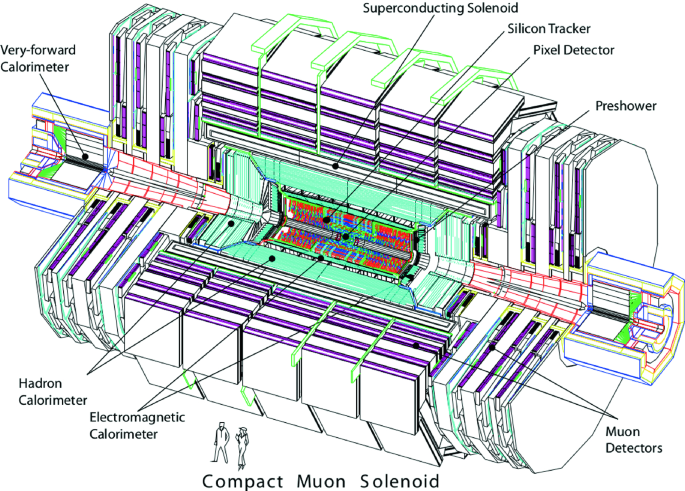
\includegraphics[width=0.7\textwidth]{ashish_thesis/cms_exp.png}
\caption{%
   Compact muon solenoid (CMS) detector with all of the sub detectors showing silicon tracker, electromagnetic and hadron calorimeters and muon chambers. 
}
\label{fig:cms}
\end{figure}




%In summary, luminosity is a critical parameter in particle physics experiments that determines the rate at which particles are produced and detected. The higher the luminosity, the greater the probability of detecting rare or low-probability events. The production rate of a particle of interest is proportional to the product of the luminosity and the cross-section of the process that produces the particle, and increasing the luminosity is essential for increasing the production rate of rare particles.Luminosity is a fundamental concept in particle physics that describes the rate at which particles collide in a particle accelerator. It is defined as the number of particles per unit time and unit cross-sectional area of the particle beams. In other words, it is a measure of the intensity of the particle beams and determines the number of collisions that occur within a given time. The importance of luminosity in particle physics lies in the fact that it directly affects the ability to detect rare events and make precise measurements. The more collisions that occur, the higher the probability of rare events happening, such as the creation of new particles or the detection of new phenomena. Additionally, precise measurements require a large number of collisions to be able to statistically determine the properties of the particles being studied. In high-energy particle accelerators, such as the Large Hadron Collider (LHC) at CERN, the luminosity is typically measured in units of inverse femtobarns ($fb^{-1}$), which is a measure of the total number of collisions per unit area during the course of an experiment. For example, the LHC has a design luminosity of $10^{34} cm^{-2}s^{-1}$, which means that there are $10^{34}$ proton-proton collisions per second per square centimeter of the detector. In order to achieve high luminosity, particle accelerators use various techniques to increase the number of particles in the beams and focus them to a small cross-sectional area. One technique is to use superconducting magnets to guide the particles along a circular path and keep them confined to a small area. Another technique is to use radio frequency cavities to accelerate the particles to higher energies. The importance of luminosity can be seen in the many discoveries that have been made in particle physics due to high-luminosity experiments. For example, the discovery of the Higgs boson at the LHC was made possible by the high luminosity of the collider, which allowed physicists to observe the rare Higgs boson signal over the background noise of other particles. In addition to discoveries, high luminosity experiments are also important for precision measurements. For example, the measurement of the properties of the top quark, the heaviest known elementary particle, requires a large number of collisions to be able to distinguish the signal from the background noise.


\section{Run 1 and Run 2 luminosity measurement}

During the operation of the CMS experiment, two main data-taking periods were conducted: Run 1, which spanned from 2010 to 2013, and Run 2, which took place from 2015 to 2018. During these periods, the CMS experiment measured the instantaneous and integrated luminosity of the proton-proton collisions produced by the Large Hadron Collider (LHC) shown in Fig.~\ref{fig:lumi}. During Run 1, the CMS experiment achieved a peak instantaneous luminosity of up to $5 \times 10^{33} cm^{-2} s^{-1}$, while during Run 2, the luminosity reached a peak value of up to $2 \times 10^{34} cm^{-2} s^{-1}$. The luminosity measurements during both runs were accompanied by careful assessments of the systematic uncertainties to ensure accurate and reliable results as shown in Table. \ref{tab:lumi}.

%\begin{tabular}{c c c c}
%Year & Center of Mass Energy (TeV) & Integrated Luminosity (fb$^{-1}$) & Systematic Uncertainty (\%) \\
%\hline
%2010 & 7 & 0.04 & N/A \\
%2011 & 7 and 8 & 5.6 & 4.5 \\
%2012 & 8 & 23.3 & 2.5 \\
%2015 & 13 & 3.8 & 2.3 \\
%2016 & 13 & 40.8 & 2.5 \\
%2017 & 13 & 49.8 & 2.3 \\
%2018 & 13 & 67.9 & 2.5 \\
%\end{tabular}

\begin{table}[h]
\centering
\caption{Summary of center of mass energy, integrated luminosity, and systematic uncertainty per year during the CMS luminosity measurement.}
\begin{tabular}{c c c c}
Year & Center of Mass Energy (TeV) & Integrated Luminosity (fb$^{-1}$) & Systematic Uncertainty (\%) \\
\hline
2010 & 7 & 0.045 & 11 \\
2011 & 7 and 8 & 6.1 & 4.5 \\
2012 & 8 & 23.3 & 2.5 \\
2015 & 13 & 4.3 & 2.3 \\
2016 & 13 & 41.6 & 2.5 \\
2017 & 13 & 49.8 & 2.3 \\
2018 & 13 & 67.9 &  2.5\\
\end{tabular}
\label{tab:lumi}
\end{table}


\begin{figure}[!htp]
\centering
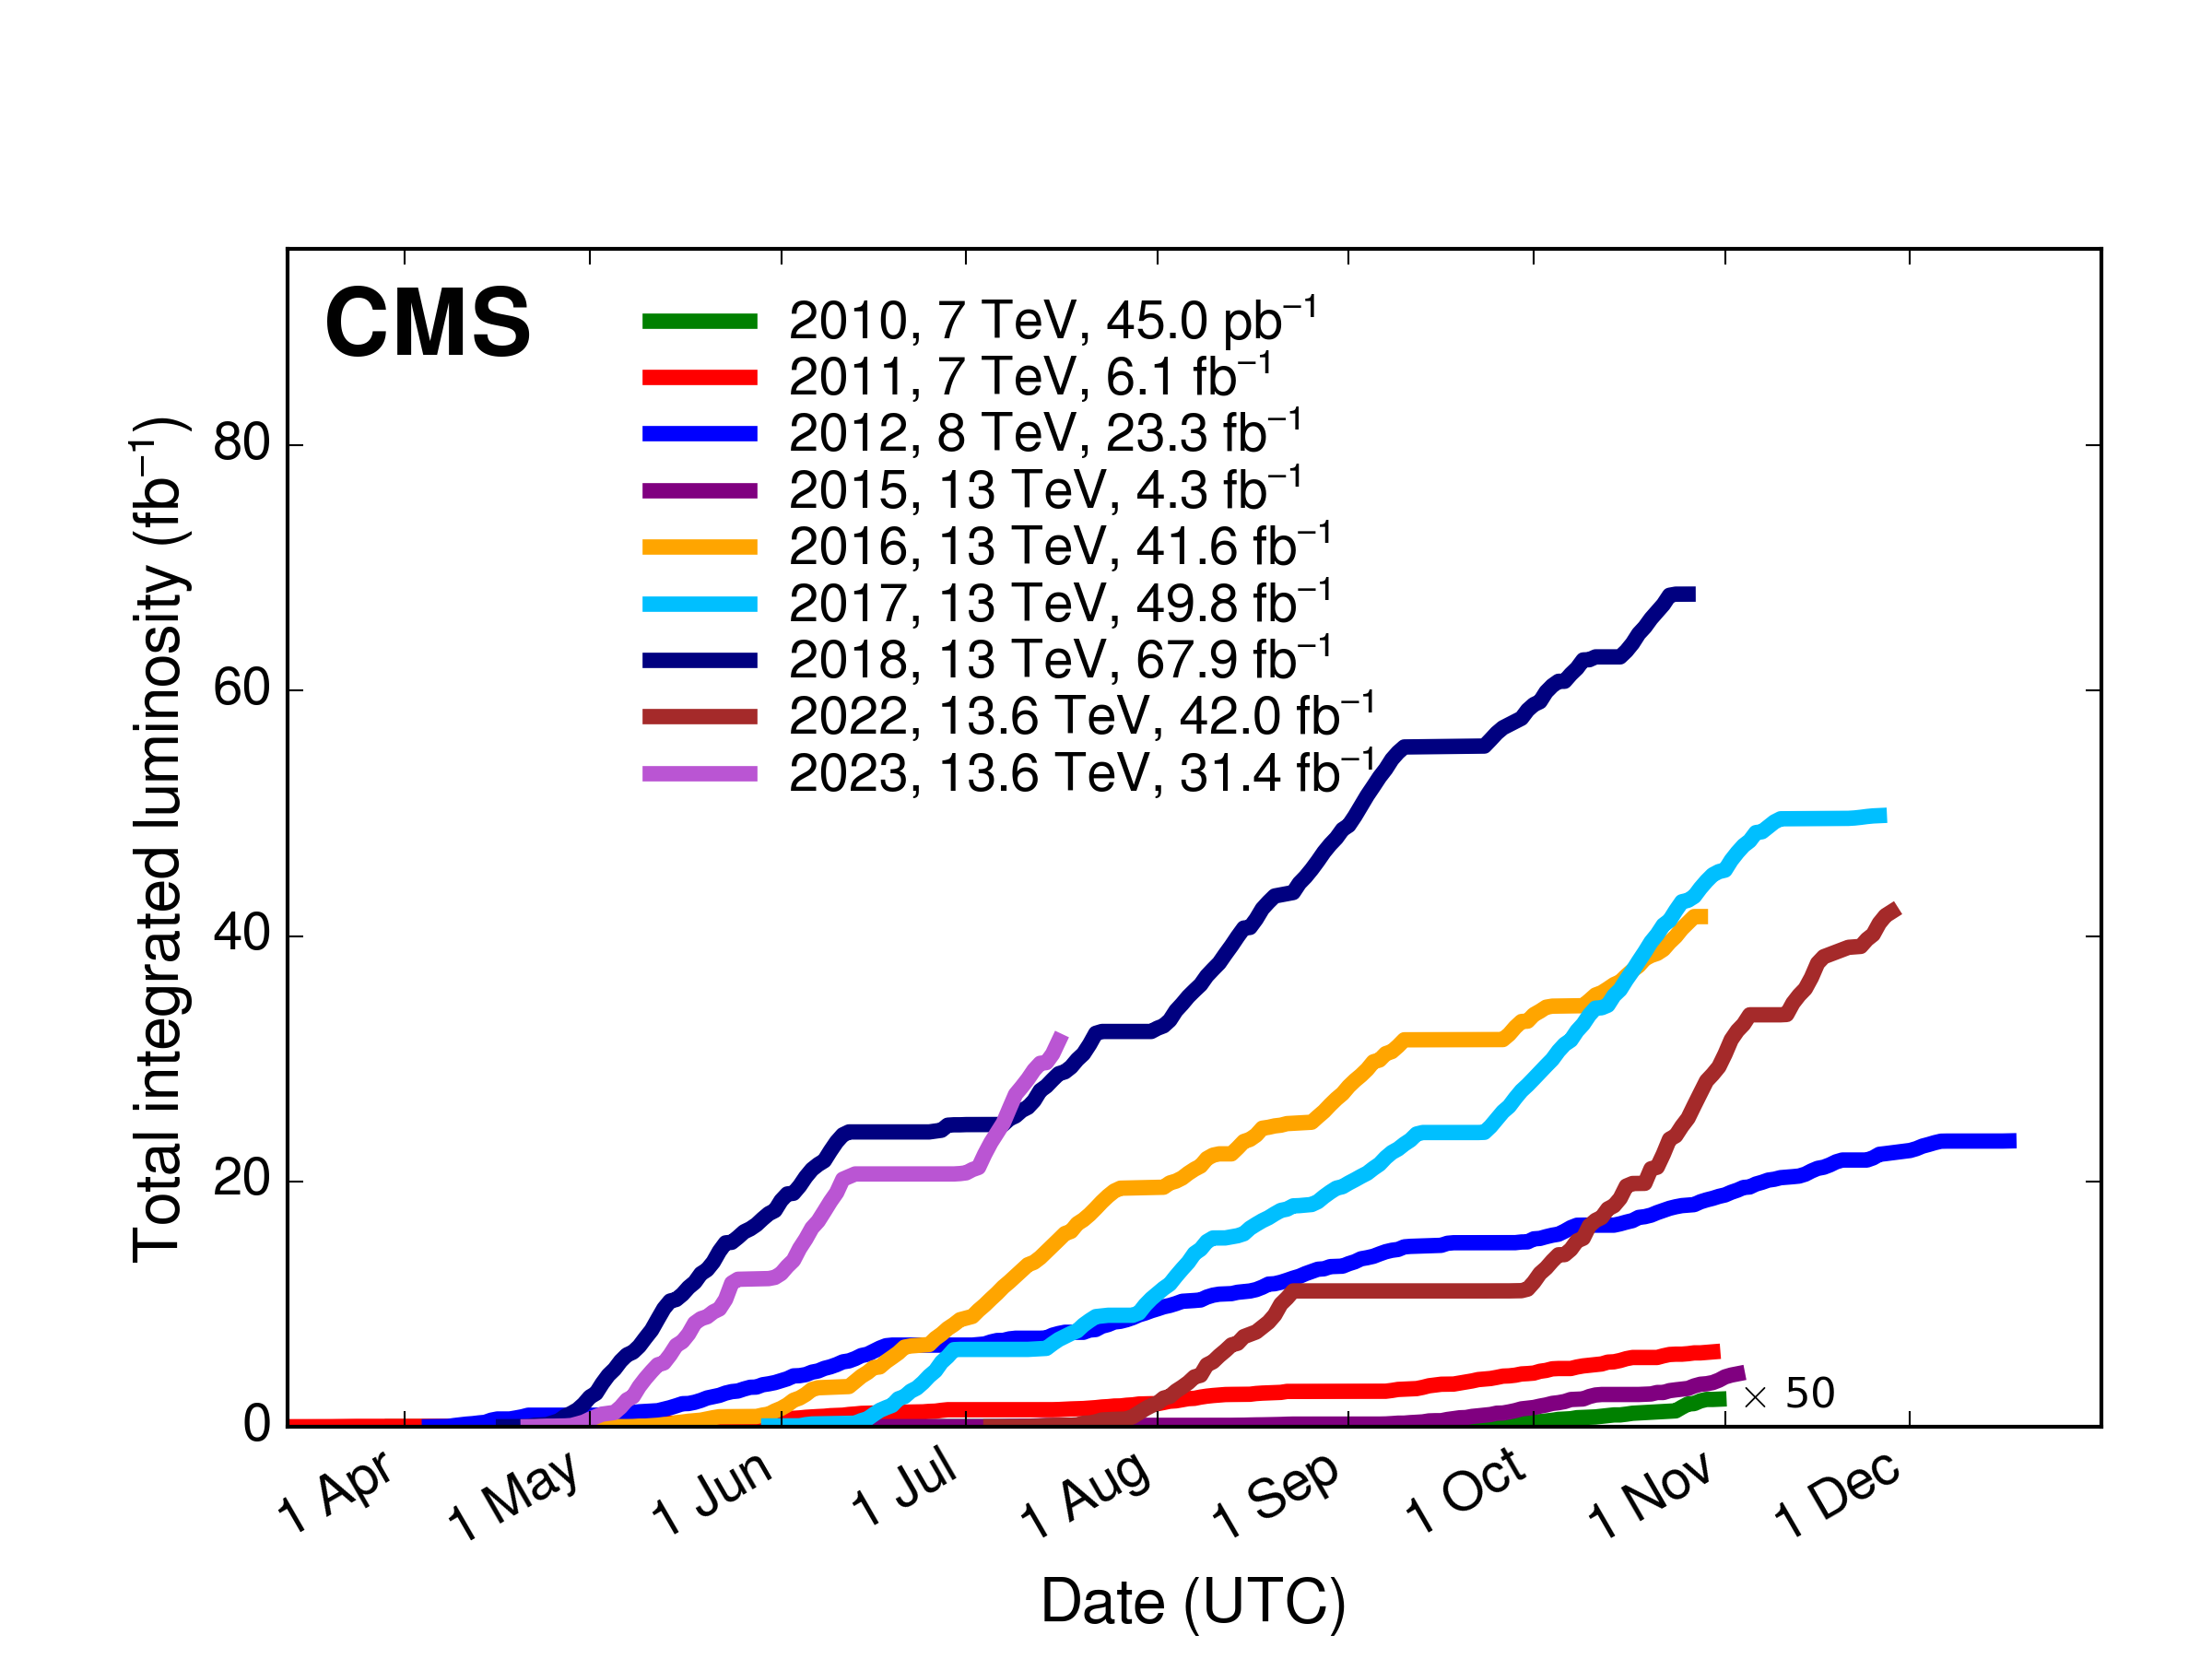
\includegraphics[width=0.8\textwidth]{ashish_thesis/CMS_luminosity.png}
\caption{%
    Delivered luminosity versus time for Run 1 and Run 2 of the CMS experiment.
}
\label{fig:lumi}
\end{figure}



